\documentclass[oneside]{article}
\usepackage{fancyhdr}
\usepackage{graphicx}
\usepackage{float}
\usepackage{enumitem}
\pagestyle{fancy}
\title{Parallel Design Patterns II}
\author{B138813}
\date{February 2019}

\begin{document}
\lhead{Parallel Design Patterns II}
\rhead{B138813}

\maketitle
\section{Introduction}
We present our report for the second submission of the Parallel Design Patterns Coursework. We first discuss our implementation in Section~\ref{sec:imp}, and demonstrate its correctness in Section~\ref{sec:cor}. Although our implementation has some features similar to a framework, we were not able to succesfully seperate policy and mechanism to an adaquete extend. We will discuss this issue further in Section~\ref{sec:fur}.



\section{Implementation}\label{sec:imp}
We implemented our squirrel simulation in C++. We present a UML diagram of our implementation in Figure~\ref{fig:uml}. To maximise code re-use, we abstracted as much common functionality into the parent actor class as possible. The actor class holds methods such as \texttt{send\_msg()} and \texttt{msg\_recv()} which act as wrappers to MPI functions, whilst also providing extra functionality. For example, \texttt{msg\_recv()} returns a three item tuple, which contains:

\begin{itemize}
  \item A boolean, which indicates if the message was succesfully recieved.
  \item An integer, which indicates where the message was recived from.
  \item An integer, which is the message itself.
\end{itemize}
The semantics of the message integer are encoded into the \texttt{MSG} enum, which is shared by all actors. This standardisation makes it easy for the programmer to reason about messages, allowing them to dictate how a message if handled in each child class's main event loop. The function \texttt{send\_msg()} is simple convenience wrapper around \texttt{MPI\_Bsend()}. Each class inherits directly from the actor class, except for the controller, which is a child of the master class. We made this decision because the master and controller share most of their functionality and variables. The master class starts the simulation, and then provides process pool functionality. The controller class keeps track of the number of live and infected squirrels.

\begin{figure}[H]
  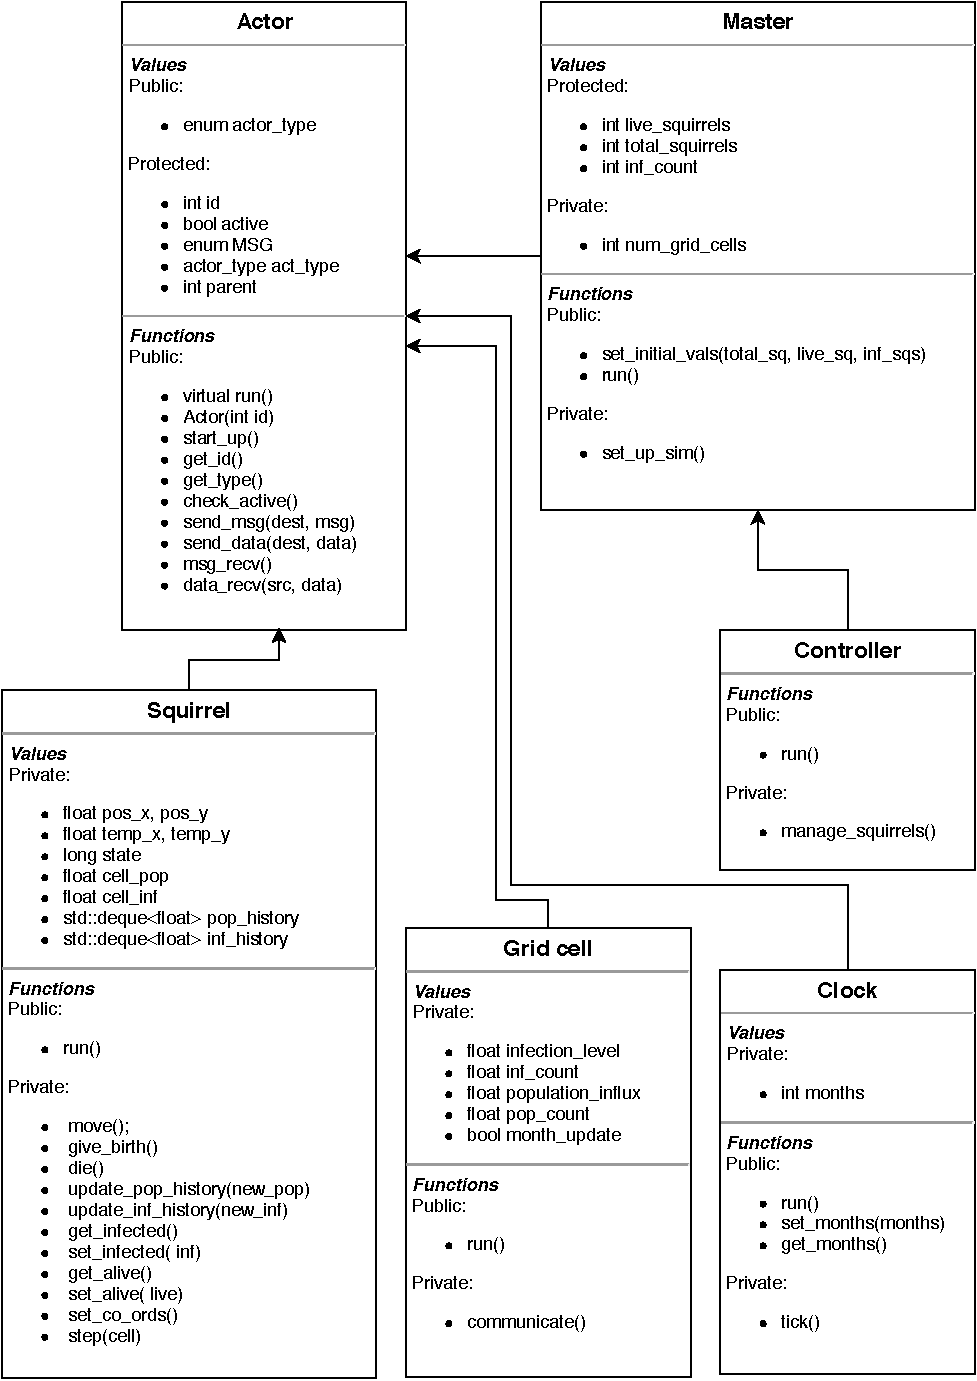
\includegraphics[width=\linewidth]{figures/pdp_uml}
  \caption{UML Diagram of the Program}
  \label{fig:uml}
\end{figure}

 Both classes need to know the simulation's initial squirrel numbers, and share functions and values to implement this. If C++'s inheritance model did not allow both child and grandchild classes to implement their own versions their parent's virtual functions, this pattern would not be possible. The squirrel class has the most functions of any class, partly because of how active the biologists model demands the squirrel to be, and partly because of how we have decided to model our actors.

 Each actor has an actor type, as designated by the enumerate type \texttt{actor\_type}. There three different actor type for squirrels; infected squirrels, dead squirrels and normal, healthy squirrels. To safely change a squirrel from one of these types to another, we thought it best to encapsulate the code within a function. In doing so, we keep our code compliant with object oriented design philosophies, but diverge from high performance programming ones. However, we do not think the addition of these functions degrades the performance of our work too much, and improves the readablity of our code.

 There are four key communications between our actors. We have endevored to abstract them and encapulate them into our actor class. We will now describe our implementations of those actors.

 \subsection{Actor Start}
 Every actor except master enters into the worker code function and calls \texttt{start\_up()}, where the actor uses a blocking recieve to get what type of actor it is from the master. This then allows the actor to move on 

\subsection{Clock tick}
We have made use of a clock actor to send messages to every grid cell every month, modelled as a period of 0.2 milliseconds. We refer to this time period message as a tick. In the grid cell's \texttt{run()} function, while it is active we call the communication function.

\subsection{Squirrel Step}

\subsection{Squirrel Birth}


\section{Correctness}\label{sec:cor}
If no squirrels are infected, the population will continually grow.

\section{Further Work}\label{sec:fur}
Further generalise data recv or make a blocking data recv for location vector.

\end{document}
